\documentclass{article}
\usepackage[utf8]{inputenc}
\usepackage[legalpaper, portrait, margin=1in]{geometry}
\usepackage{hyperref}
\usepackage{tikz}
\usepackage{xcolor}

\title{First Proposal - EU Cybercrime}
\author{Tristan Goodell}
\date{September 2019}

\begin{document}
\tikz[remember picture,overlay] \node[opacity=1,inner sep=0pt] at (current page.center){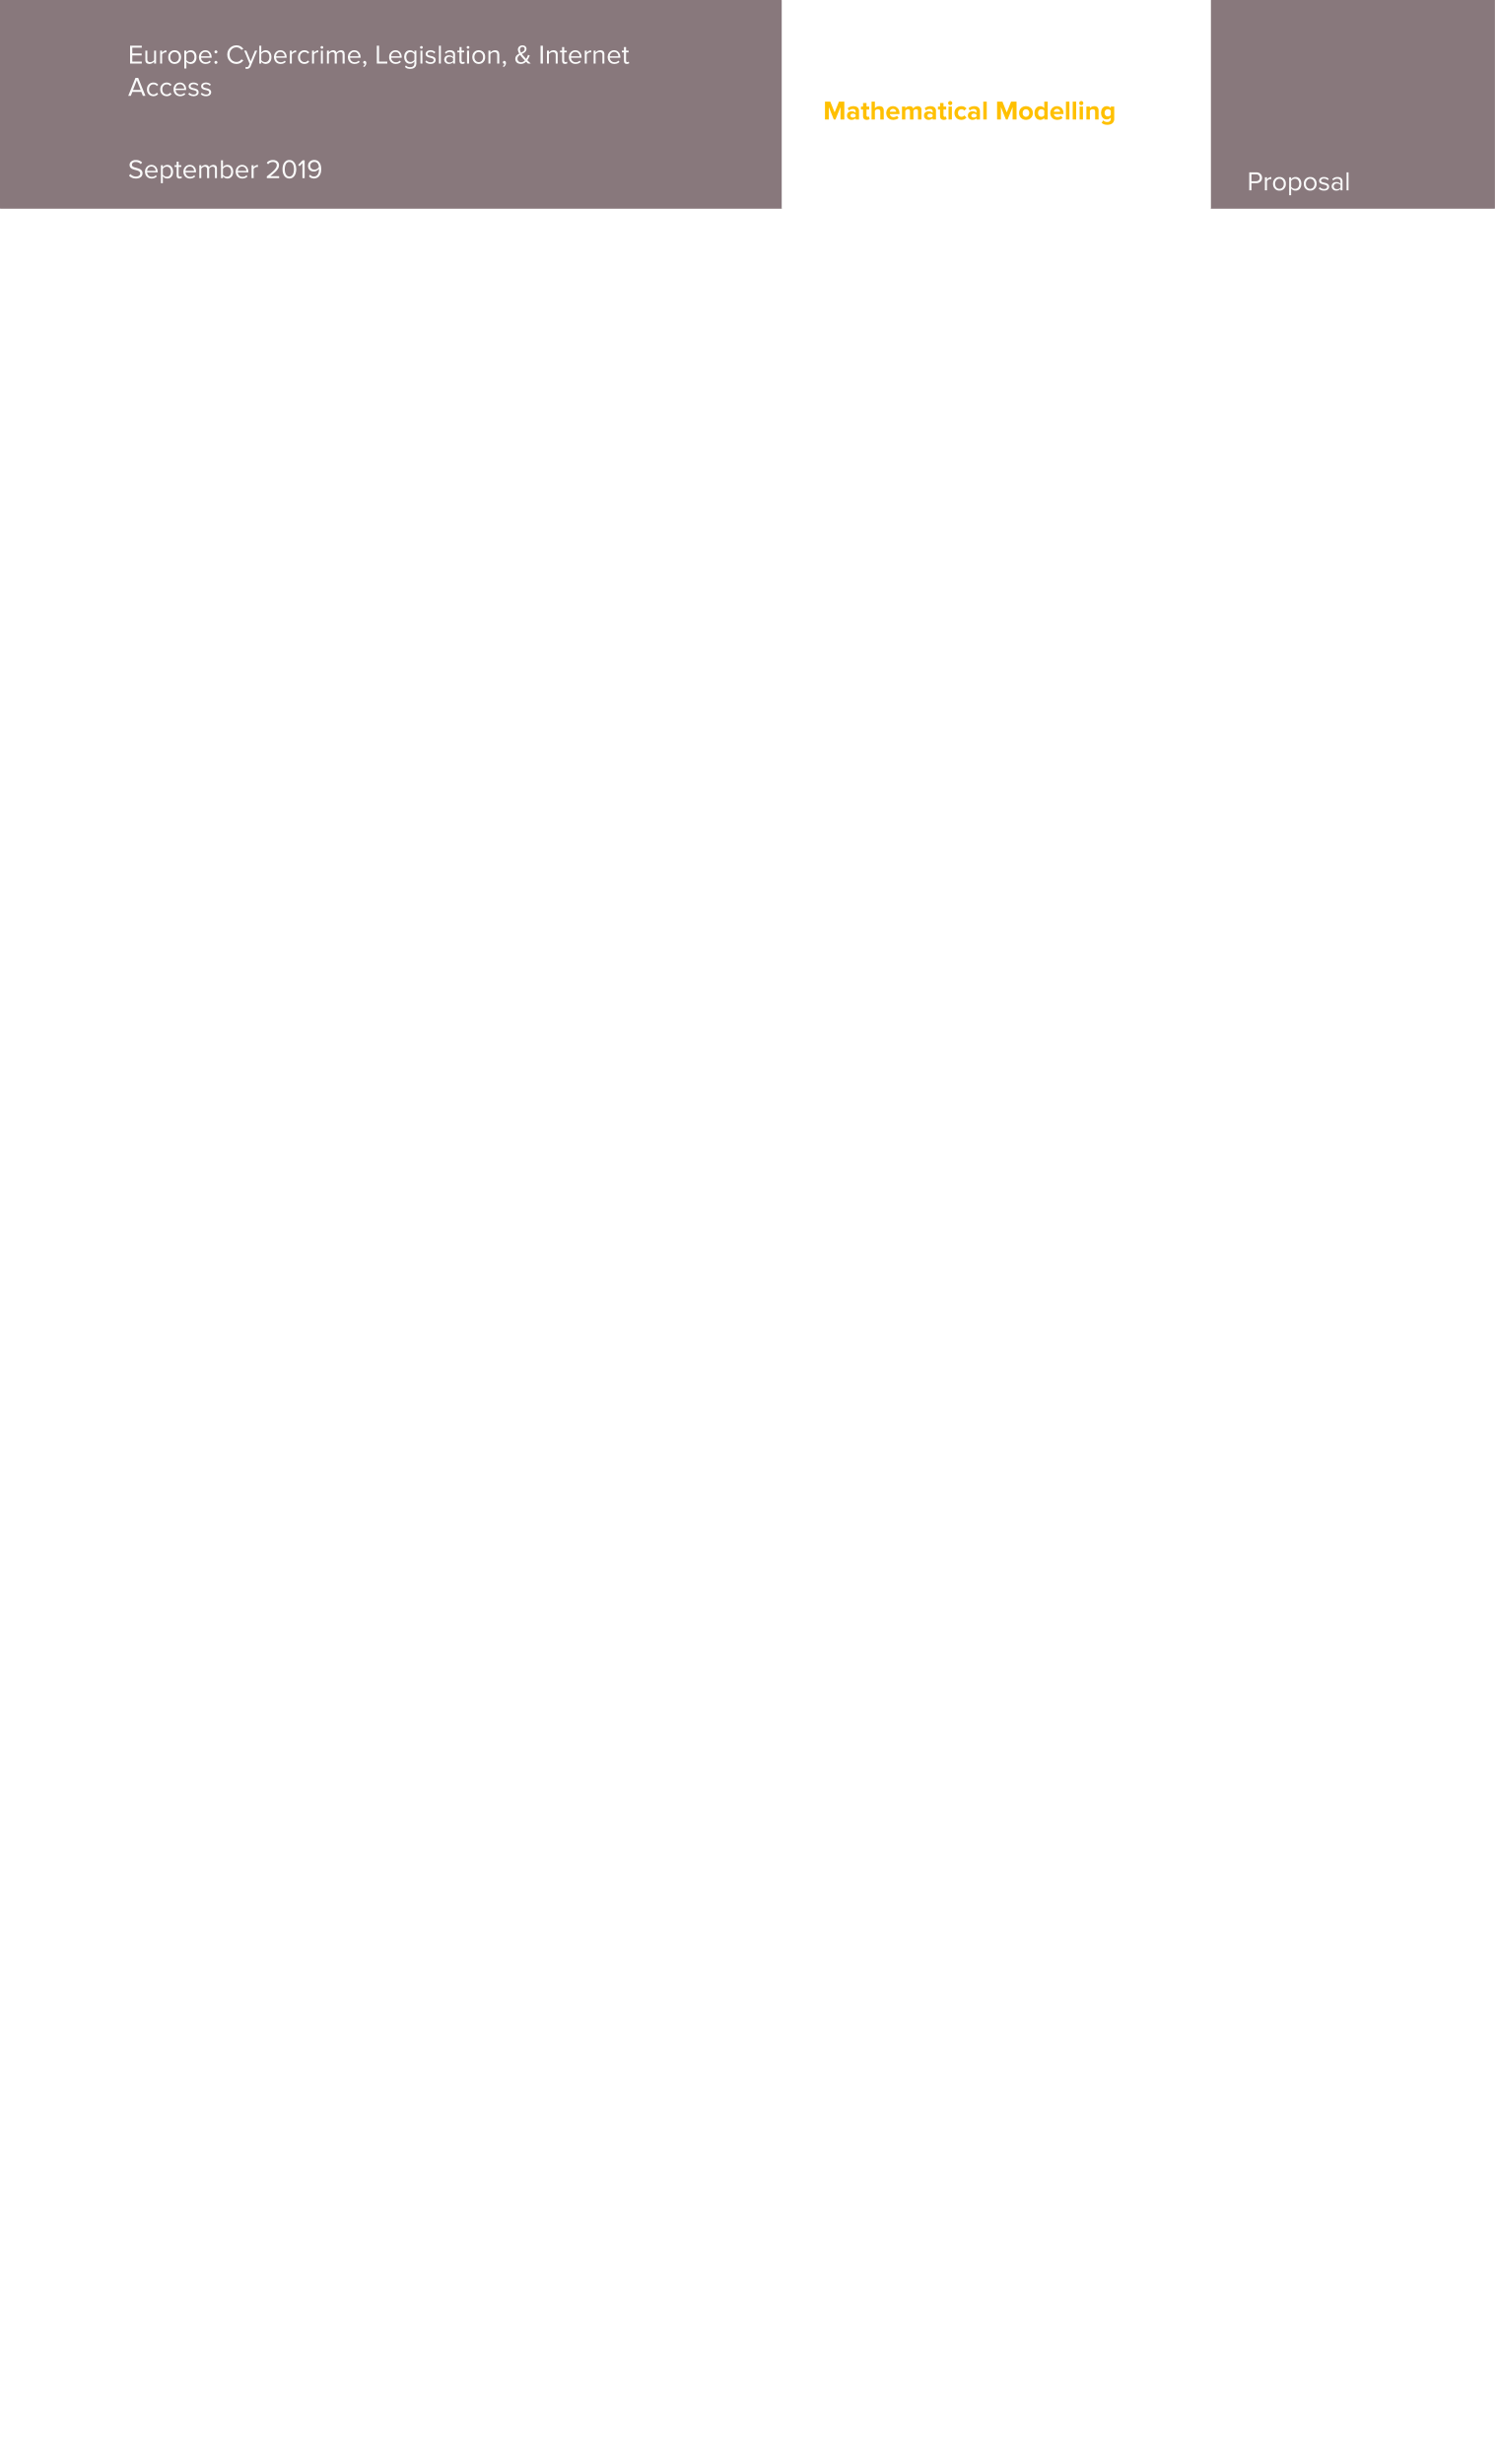
\includegraphics[width=\paperwidth]{ProposalBackground.png}};
\definecolor{EUblue}{HTML}{365f91}


{\color{EUblue}\section{Rationale}}

This project has been proposed to:

\begin{itemize}
    \item Analyze the correlation between perception of cybercrime and actual cybercrime.
    \item Display the relationship between internet access/use and various factors, such as country.
    \item Determine the effect EU legislation has had on the perception of cybercrime.
    \item Establish a timeline consisting of all major data breaches, privacy scandals, EU Legislation, internet market penetration, and perception of cybercrime from 2012 to 2018. 
\end{itemize}

This project will allow the European Union to better understand cybercrime and a history of the public opinion of cybercrime in addition its correlation with a variety of factors, including country, legislation, data breaches, etc. This is possible thanks to the Eurobarometers from 2012, 2013, 2015, 2017, and 2019 (EU public opinion) and other EU funded reports regarding cybercrime. 

{\color{EUblue}\section{Research Goals}}

The goal of this project is to determine if EU legislation, in addition to other EU funded endeavors, have an effect on the perception of cybercrime in the EU, actual cybercrime in the EU, and internet access for EU citizens. 

\vspace{\baselineskip} 

{\color{EUblue}\section{Procedure}}

\begin{itemize}
    \item Phase I: I will finish gathering reports of interest from the European Commission in order to have enough information regarding European public opinion on cybercrime, internet accessibility, and statistics regarding cybercrime in the EU. This information will then be compiled into a spreadsheet for easy analysis in Excel or R. 
    \item Phase II: The data will be analyzed using relevant statistical tools including, but not limited to, T-Tests, Z-Tests, ANOVA, T-Intervals, Z-Intervals, and the Coefficient of Determination. 
    \item Phase III: Mathematical Models will then be created using the data gathered in Phase I and the findings in Phase II. Further, a timeline, consisting of EU legislation, EU public opinion of cybercrime, cybercrime statistics, and other developments in cyber security and privacy, will be constructed. 
    \item Phase IV: I will finally write the paper in LaTeX. The findings in Phase II and the models constructed in Phase III will be included in addition to an overall background of cybercrime in the EU (since most readers will be familiar with US cybercrime). 
    \item Phase V: Present at Science Fair. 
\end{itemize}

{\color{EUblue}\section{Bibliography}}

\begin{itemize}
    \item European Union Directorate-General for Communication. “Special Eurobarometer 390: ‘Cyber Security.’” , European Commission, July 2012, \href{https://ec.europa.eu/commfrontoffice/publicopinion/index.cfm/Survey/getSurveyDetail/instruments/SPECIAL/surveyKy/1058}{ec.europa.eu...}.
    \item European Union Directorate-General for Communication. “Special Eurobarometer 404: ‘Cyber Security.’” European Commission, Nov. 2013, \href{https://ec.europa.eu/commfrontoffice/publicopinion/index.cfm/Survey/getSurveyDetail/instruments/SPECIAL/surveyKy/1073}{ec.europa.eu...}
    \item European Union Directorate-General for Communication. “Special Eurobarometer 423: ‘Cyber Security.’” European Commission, Oct. 2015, \href{https://ec.europa.eu/commfrontoffice/publicopinion/index.cfm/Survey/getSurveyDetail/instruments/SPECIAL/surveyKy/2019}{ec.europa.eu...}
    \item European Union Directorate-General for Communication. “Special Eurobarometer 464a: ‘Europeans’ attitudes towards Internet security.’” European Commission, Sept. 2017, \href{https://ec.europa.eu/commfrontoffice/publicopinion/index.cfm/Survey/getSurveyDetail/instruments/SPECIAL/surveyKy/2171}{ec.europa.eu...}.
    \item European Union Directorate-General for Communication. “Special Eurobarometer 480: ‘Europeans’ attitudes towards Internet security.’” European Commission, March 2019, \href{https://ec.europa.eu/commfrontoffice/publicopinion/index.cfm/survey/getsurveydetail/instruments/special/surveyky/2207}{ec.europa.eu...}.
    \item Migration and Home Affairs. “Cybercrime.’” European Commission, \href{https://ec.europa.eu/home-affairs/what-we-do/policies/cybercrime_en}{ec.europa.eu...}.
    \item European Commission. Cybersecurity,’” European Commission, August 2019, \href{https://ec.europa.eu/digital-single-market/en/cyber-security}{ec.europa.eu...}.
    \item Europol. Internet Organised Crime Threat Assessment 2018,’” Europol, 2018, \href{https://www.europol.europa.eu/internet-organised-crime-threat-assessment-2018}{europol.europa.eu...}.
\end{itemize}
\end{document}
